\documentclass[tikz, border=1mm]{standalone}

\tikzstyle{plot_adiar} =[color=cyan,   opacity=0.8, mark=o,        mark size=0.5pt, line width=0.9pt]
\tikzstyle{plot_buddy} =[color=orange, opacity=0.7, mark=triangle, mark size=0.4pt, line width=0.7pt]
\tikzstyle{plot_cal}   =[color=purple, opacity=0.7, mark=+,        mark size=0.9pt, line width=0.9pt]
\tikzstyle{plot_cudd}  =[color=orange, opacity=0.7, mark=diamond,  mark size=0.4pt, line width=0.7pt]
\tikzstyle{plot_sylvan}=[color=orange, opacity=0.7, mark=square,   mark size=0.4pt, line width=0.7pt]

% graphics
\usepackage{color}
\usepackage{tikz}
\usepackage{graphicx}
\usepackage{pgfplots}
\pgfplotsset{compat=1.16}
\usepgfplotslibrary{fillbetween}

\begin{document}

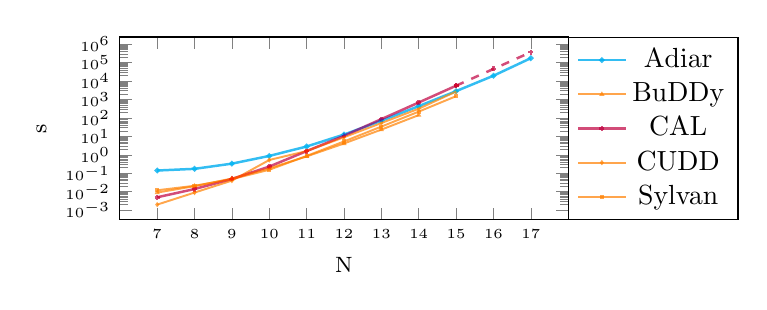
\begin{tikzpicture}
  \begin{axis}[%
    width=0.6\linewidth,
    height=0.322\linewidth,
    every tick label/.append style={font=\tiny},
    % x-axis
    xlabel={\footnotesize N},
    xmajorgrids=false,
    xtick={7,...,17},
    % y-axis
    ylabel={\footnotesize s},
    ytick distance={10},
    ymode=log,
    yminorgrids=false,
    ymajorgrids=false,
    grid style={dashed,black!5},
    % legend
    legend style={at={(1,1.001)}, anchor=north west},
    ]

    \begin{scope}[blend mode=soft light]
      % depth-first implementations
      \addplot+ [style=plot_buddy, forget plot] coordinates {
        (7,  0.009)
        (8,  0.020)
        (9,  0.052)
        (10, 0.186)
        (11, 0.821)
        (12, 4.117)
        (13, 23.255)
        (14, 142.423)
      };

      \addplot+ [style=plot_cudd, forget plot] coordinates {
        (7,  0.002)
        (8,  0.009)
        (9,  0.040)
        (10, 0.526)
        (11, 1.593)
        (12, 8.967)
        (13, 52.881)
        (14, 316.093)
        (15, 2687.585)
      };

      \addplot+ [style=plot_sylvan, forget plot] coordinates {
        (7,  0.012)
        (8,  0.021)
        (9,  0.048)
        (10, 0.155)
        (11, 0.868)
        (12, 5.321)
        (13, 33.840)
        (14, 219.785)
        (15, 1508.866)
      };

      % breadth-first implementations
      \addplot+ [style=plot_cal, forget plot] coordinates {
        (7,  0.005)
        (8,  0.014)
        (9,  0.049)
        (10, 0.231)
        (11, 1.592)
        (12, 10.696)
        (13, 86.135)
        (14, 685.696)
        (15, 5580.124)
      };
      \addplot+ [style=plot_cal, dashed, forget plot] coordinates {
        % Projection, assuming CAL does not slow down due to swap memory.
        (15, 5580.124)
        (16, 45198)
        (17, 366103.8)
      };

      % time-forward processing, i.e. Adiar
      \addplot+ [style=plot_adiar, forget plot] coordinates {
        (7,  0.141)
        (8,  0.174)
        (9,  0.333)
        (10, 0.871)
        (11, 2.828)
        (12, 12.530)
        (13, 70.100)
        (14, 434.766)
        (15, 2829.750)
        (16, 19400.135)
        (17, 173650.677)
      };

      % legend
      \addlegendimage{plot_adiar};
      \addlegendentry{Adiar};

      \addlegendimage{plot_buddy};
      \addlegendentry{BuDDy};

      \addlegendimage{plot_cal};
      \addlegendentry{CAL};

      \addlegendimage{plot_cudd};
      \addlegendentry{CUDD};

      \addlegendimage{plot_sylvan};
      \addlegendentry{Sylvan};
    \end{scope}
  \end{axis}
\end{tikzpicture}

\end{document}